\section{Experimental Design}
\subsection{Corpus, annotations, and audit}
The frozen snapshot contains 418 source images: 297 Magnolia and 121 Azalea. Five zero-width annotation rows are rejected without modifying the reviewed labels, leaving 29,842 one-class plant boxes (15,644 Magnolia and 14,198 Azalea). Three reviewed Azalea sources contain no instances and are retained as source-level negatives; one unmatched RGB frame is excluded. With $1024\!\times\!1024$ tiles, $.25$ overlap, and minimum box visibility $.5$, preparation yields 14,630 tiles, including 1,328 boundary-aware empty candidates.

\begin{table}[t]
\centering
\wacvtablefont
\caption{Frozen corpus and source-safe split. Human-audit and detector columns remain blocked until their artifacts are verified.}
\label{tab:data}
\setlength{\tabcolsep}{3.5pt}
\begin{tabular}{lrrrrr}
\toprule
Crop & Sources & Boxes & Train/Val/Test & Audit & Det. rec. \\
\midrule
Magnolia & 297 & 15,644 & \pendingcell & \pendingcell & \pendingcell \\
Azalea & 121 & 14,198 & \pendingcell & \pendingcell & \pendingcell \\
\midrule
Total & 418 & 29,842 & 302/58/58 & \pendingcell & \pendingcell \\
\bottomrule
\end{tabular}
\end{table}

A frozen human audit stratifies by crop, source, normalized box size, image boundary, annotation density, and negative status. The final report will state sample size, reviewer count, agreement, adjudication, and exclusions. Exact and perceptual duplicate checks operate at source level; source, sequence, flight, or row identifiers are grouped when metadata permit. Split and manifest hashes are recorded before model evaluation.

\subsection{Observed domain shift}
Azalea contains a higher median annotated count per source than Magnolia and a smaller median normalized box area. Appearance and green-fraction distributions also differ. Figure~\ref{fig:domainshift} describes these measured marginals before model fitting; it motivates directed evaluation but is not treated as causal proof of transfer error.

\begin{figure*}[t]
    \centering
    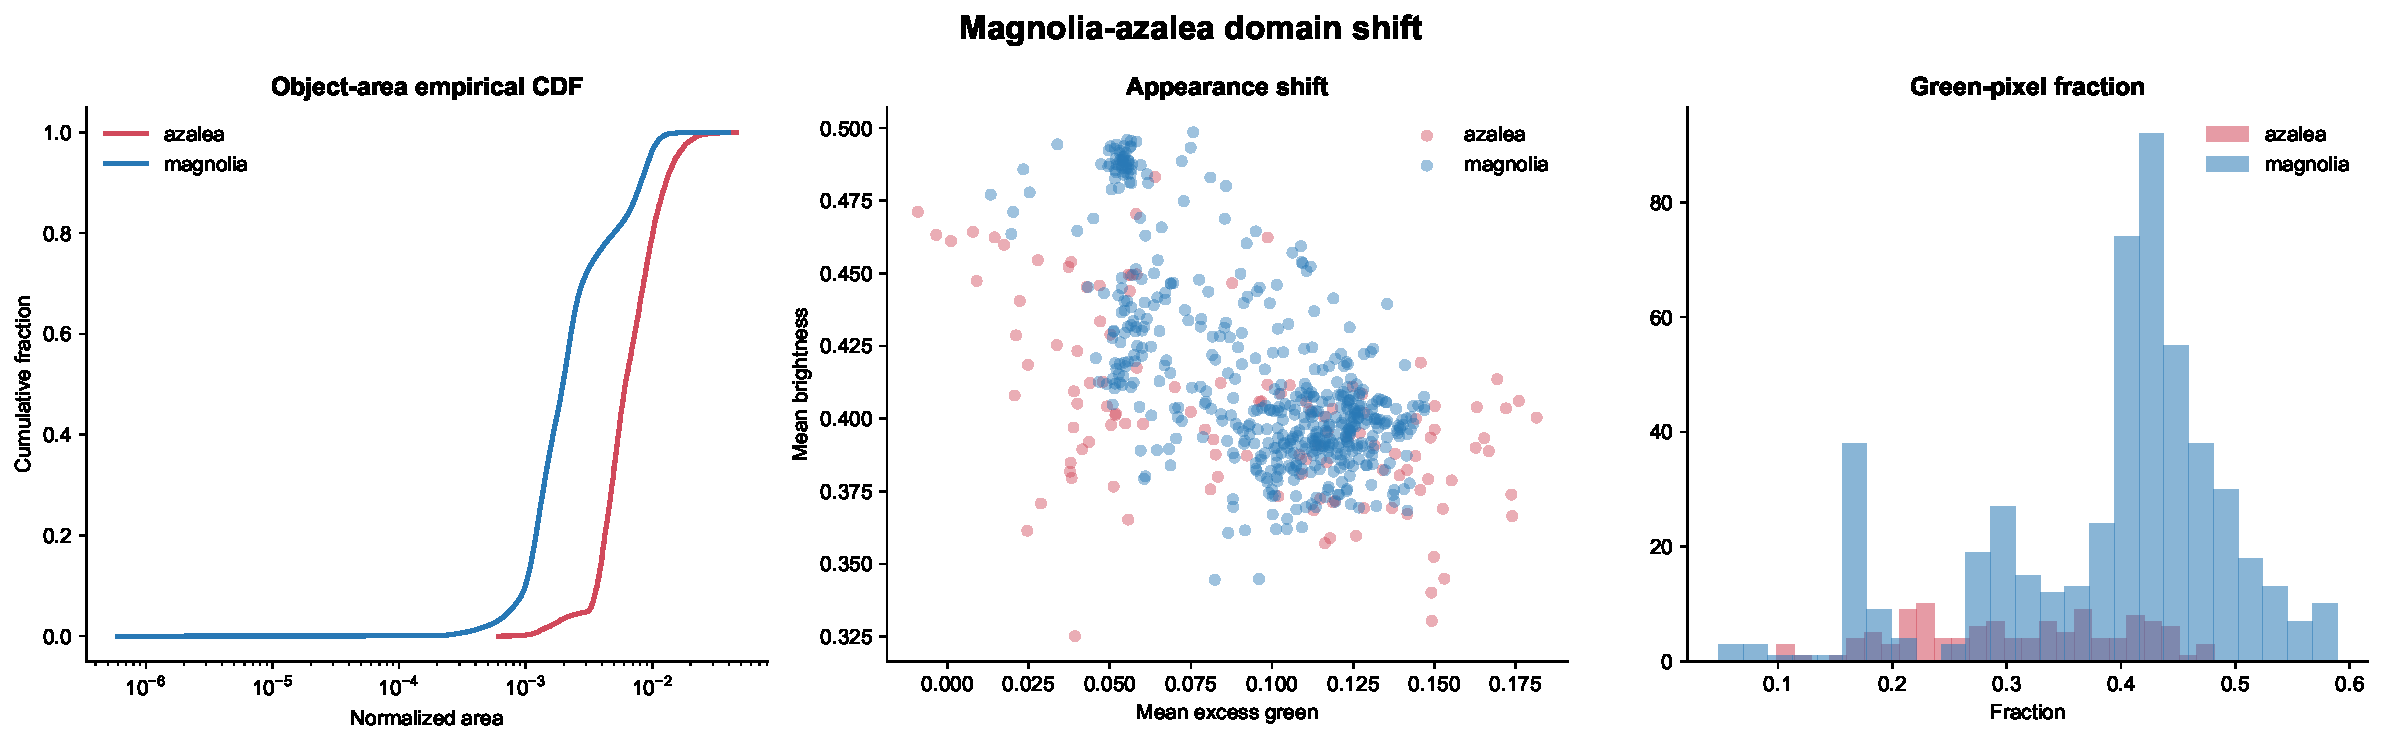
\includegraphics[width=\textwidth]{figures/cross_crop_shift.pdf}
    \caption{\textbf{Measured Magnolia--Azalea shift.} Object geometry uses valid source boxes; appearance statistics are computed once per source. No model prediction enters the figure. The corresponding directed transfer results are reported separately.}
    \label{fig:domainshift}
\end{figure*}

\subsection{Tasks and source-level targets}
Presence is positive when a source contains at least one verified instance. Count is evaluated continuously by mean absolute error and categorically using intervals fitted on training sources only. Density and annotated coverage use training-only thresholds with adequate support in every evaluated class; otherwise they remain continuous or diagnostic outcomes. The primary endpoint is strict source-record correctness: all required inventory fields must be correct. Per-field macro-F1, count error, and coverage error are secondary endpoints. A malformed record is incorrect rather than silently repaired.

\subsection{Directed evaluation protocols}
We evaluate Magnolia$\rightarrow$Magnolia (M$\rightarrow$M), Azalea$\rightarrow$Azalea (A$\rightarrow$A), M$\rightarrow$A, A$\rightarrow$M, and crop-stratified pooled training. Here transfer refers explicitly to every fitted component: detector, ranking parameters, reducer, and gate. The VLM checkpoint remains frozen. Target-crop test labels are used only for final scoring. Tile parameters, prompt, schema, risk target, and all component choices are frozen without target-test feedback. Method comparisons on the same target sources use paired resampling; differences between distinct Magnolia and Azalea test sets are domain gaps and are not called paired effects.

\subsection{Controlled systems and baselines}
The primary VLM is chosen on validation evidence before test scoring. SmolVLM2-500M, SmolVLM2-2.2B, Phi-3.5-Vision, and LLaVA-1.5-7B form a secondary model ladder. All VLMs receive the same source tiles, semantic prompt, output schema, generation-token cap, and stopping rule. Because native image processors differ, processed tensor resolution and visual-token count are recorded rather than described as identical visual input.

The system comparison includes: (i) detector-only source aggregation; (ii) deterministic detector-derived inventory rules; (iii) one whole-image downsampled VLM input; (iv) uniformly tiled VLM inference at budget $K$; and (v) detector-routed VLM inference with and without selective review. Routing policies are random, true coordinate-aware spatial selection, confidence top-$K$, count top-$K$, normalized combined top-$K$, exploit--explore, and diversity-aware exploration. Shuffled scores and GT-oracle routing are diagnostic controls only.

Reliability baselines are raw VLM confidence, strict-schema rejection, detector agreement, an equal-weight fixed score, and the cross-fitted learned gate. Comparisons are made at matched coverage and at one validation-declared target risk.

\subsection{Metrics, uncertainty, and efficiency}
For test sources ordered by increasing predicted risk, let $e_{(j)}$ indicate strict source-record error. Selective risk and area under the risk--coverage curve are
\begin{equation}
R_m=\frac{1}{m}\sum_{j=1}^{m}e_{(j)},\qquad
\mathrm{AURC}=\frac{1}{N}\sum_{m=1}^{N}R_m.
\label{eq:aurc}
\end{equation}
We also report coverage at the declared target risk, observed accepted risk, false acceptance on verified negative sources, accepted-source count, and review rate. Routing diagnostics are evidence recall, spatial coverage, overlap redundancy, boundary truncation, negative retention, and selected-negative fraction.

All intervals use source-clustered bootstrap resampling, or a higher acquisition group when flight/block metadata show dependence. Policy and model comparisons on shared target sources use paired bootstrap differences; marginal interval overlap is not used as a significance test. Stochastic routing uses order-invariant per-source seeds and repeated runs. Hyperparameters and policy selection use validation data only.

Efficiency is measured from source decoding to final decision: tiling, detector inference, selection, image preparation/transfer, VLM generation, parsing, gating, and reduction. Timings use synchronized devices, declared batching, warm-up, repeated source-level measurements, and explicit model-loading inclusion/exclusion. We report mean and p95 source latency, throughput, peak host and accelerator memory, model-loading memory, VLM calls and generations per source, and expected review workload on named hardware and software revisions. Per-tile p95 values are never multiplied to approximate source-level p95.

\subsection{Numerical provenance}
Every table and figure is generated from immutable artifacts recording the Git commit, command, dataset and split hashes, model revision, checkpoint hash, seed, hardware, software environment, and output hash. Values in this working draft remain pending until that record is complete. The held-out test set is evaluated once after the primary configuration is frozen.
